\leadchapter{
  This chapter is a general introduction to Hawkes processes and the challenges explored in this manuscript.
  After a succinct presentation of Hawkes processes with excitation, 
  we contextualise the state-of-the-art literature concerning estimation methods in Section~\ref{sec:chap0_introduction} and present the main questions that guide our research. 
  This allows us to exhibit the two paradigms that are studied in this work: inhibition and imperfect data. 
  Section~\ref{sec:chap0_inhibition} pertains to the parametric estimation of both univariate and multivariate Hawkes processes with potential inhibiting interactions (detailed in Chapters~\ref{chapter:univariate_inhibition} and \ref{chapter:multivariate_inhibition}).
  Section~\ref{sec:chap0_missing_data} presents our contributions to the study of imperfectly observed exciting Hawkes processes (detailed in Chapters~\ref{chapter:spectral_superposition} and \ref{chapter:spectral_thinning}).
  A general outline of this manuscript is described in Section~\ref{sec:chap0_outline}.% along with the main questions that guided our research.
}

\chapter{Introduction}

\section{Statistics for Hawkes processes}\label{sec:chap0_introduction}
    \subsection{The self-exciting point process}
    %\textbf{Point processes.}
    In probability and statistics, modelling random collections of points in a certain space is commonly done through a point process.
    When studying point processes on the real line $\RR$ (or the half line $\RR_{\geq 0}$), the natural order of this space often incurs an ordering of any countable sequence of points $(T_k)_{k\in\ZZ}$: we talk then of \emph{temporal} point processes.

    In statistics, it is a common question to analyse the dynamics describing the occurrences of a certain phenomenon: the time of arrival of buses at a bus stop, the apparition of symptoms in a population or earthquake incidents in a region of the world.
    The simplest model for point processes is the homogeneous Poisson process, where the waiting times between any two event times are i.i.d\ distributed as an exponential random variables with parameter $\lambda > 0$, known as the intensity of the process.
    A natural extension of this model is obtained by allowing the intensity to be a deterministic non-negative function $\lambda:\RR \to \RR_{\geq0}$, adding a temporal dependence on point arrivals.

    \subsubsection{The Hawkes process}
    In 1971, Alan G. Hawkes introduces a past-dependent model, initially called self-exciting point processes \parencite{Hawkes1971}, which will later be known as the Hawkes point process.
    Let $\mathcal{H}_t = \sigma(\{T_k \mid k\in\ZZ, T_k \leq t\})$ denote the past history of a process $N$ for any $t\in\RR$, we define the conditional intensity function $\lambda:\RR\to\RR_{>0}$ of this process as:
    \[        \lambda(t \mid \mathcal{H}_t) = \lim_{h \to 0}{\frac{\EE[N([t,t+h]) \mid \mathcal{H}_t]}{h}}\,.
    \]
    The Hawkes process is then defined by the following expression of the conditional intensity function:
    \begin{equation}\label{eq:chap0_univariate_linear_intensity}
        \lambda(t\mid \mathcal{H}_t) = \mu + \sum_{T_k \leq t}{h(t-T_k)}\,.
    \end{equation}

    \begin{remark}
      In the literature, it is common to omit writing the history $\mathcal{H}_t$ as it is directly implied that $\lambda$ has access to the entire past of the process.
      We follow this convention throughout this work, unless marked otherwise.
    \end{remark}

    The term $\mu$ is often referred to as the baseline intensity which dictates a constant rate of occurrences, similar to a homogeneous Poisson process. 
    The dependence on the past is represented by the second term in Equation~\eqref{eq:chap0_univariate_linear_intensity}, where each event time that precedes $t$ contributes to the intensity function through the interaction function $h:\RR_{\geq0}\to\RR_{\geq0}$, also calles the kernel.

    Positivity of $h$ represents an excitation effect between points: each point $T_k$ in the past increases the value of the intensity function, which in turn increases the rate at which points in the future appear.
    For stability reasons, $h$ is assumed to converge to $0$ as $t\to+\infty$, representing the rate at which the effects from the past are ``forgotten''.

    Different shapes of $h$ allow to account for different effects. 
    On the one hand, strictly decreasing functions such as exponential \parencite{Ozaki1979, Ogata1988} or power-law kernels \parencite{Zhang2016} represent instantaneous effects, which appear as spikes in the conditional intensity function (Equation~\eqref{eq:chap0_univariate_linear_intensity}). 
    On the other hand, Rayleigh or gamma kernels \parencite{Lesage2022}, where the maximum of the function is not at the origin $t=0$, can be chosen to represent delayed effects. Figure~\ref{fig:chap0_two_kernel_examples} illustrates two Hawkes processes with two different kernels.
    The properties of the conditional intensity function are intrinsically connected to those of $h$, and so when working in parametric settings, the choice of the kernel is essential and comes with its advantages and inconveniences.
    %The choice of smooth functions is transcribed as smoothness between two consecutive event times whereas the choice of kernels with bounded supports allow to leverage results from renewal process theory.

    \begin{figure}[!ht]
        \centering
          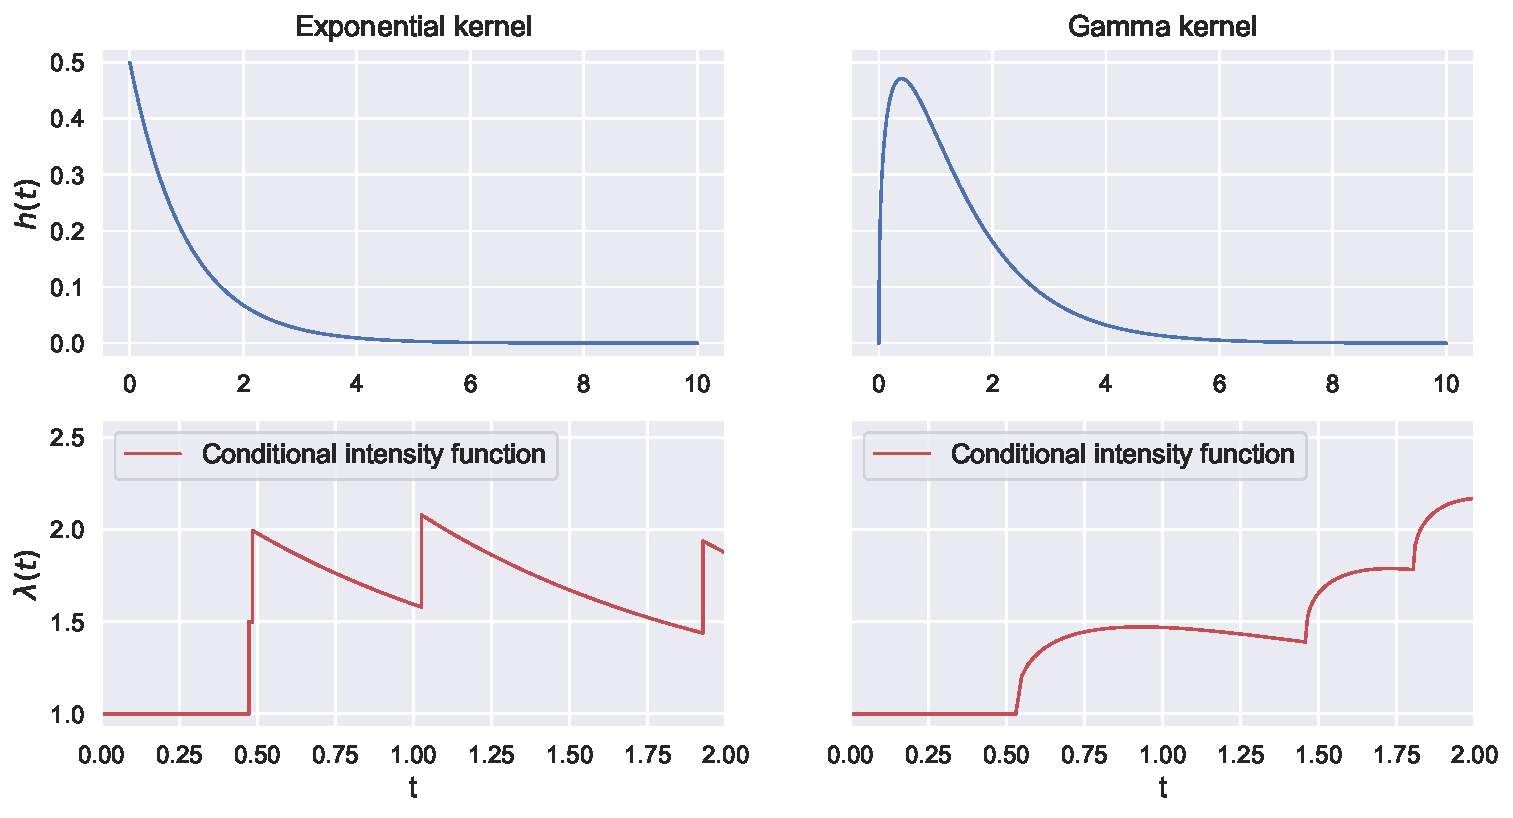
\includegraphics[width=\textwidth]{images/chapter0/two_kernel_examples_rev.pdf}
        \caption{Kernel functions (top) and respective conditional intensity functions (bottom) of a Hawkes process started at $t=0$ with baseline intensity $\mu=1$.% for exponential (left) and gamma (right) interaction functions.
        }
        \label{fig:chap0_two_kernel_examples}
      \end{figure}

    \subsubsection{Clustering and branching structures}
    A direct consequence of the expression of the intensity function (Equation~\eqref{eq:chap0_univariate_linear_intensity}) is that the Hawkes process model can be interpreted as a Poisson cluster process \parencite{Hawkes1974}.
    The most practical way of defining a cluster process \parencite{Bartlett1963} is from a generative point of view.
    We begin by simulating a homogenenous Poisson process on the real line $\RR$ with parameter $\mu$: these points $T_k^c$ are often called ancestors, immigrants or cluster centers.
    Each ancestor generates an inhomogeneous Poisson process with intensity function $h(\cdot - T_k^c)$, forming a family of children points, also called descendants.
    The iteration is repeated with each new point generating its own subprocess until no descendants are generated.
    In the end, the cluster process is formed by the union of both ancestors and descendants.
    The particularity of a Hawkes process is that the support of the function $h$ is a subset of $\RR_{\geq0}$, meaning that each occurrence influences solely the future of the process.

    This kind of process is also known as the Poisson branching process \parencite{Lewis1964} as it describes a generation dynamic similar to the Galton-Watson branching process (see \textcite{Watson1875} for the discrete time version and \textcite[Chapter III]{Harris02} for the generalised version).
    More precisely, the Hawkes process can be seen as a time-continuous branching process with immigration:
    let us assume we observe the arrival of an immigrant at a time $T_k^c$.
    This immigrant will produce a first generation of children, forming the first set of points, or branches.
    Then, each child becomes a parent and generates a new set of branches.
    A tree is then formed by the union of each immigrant and all of its branches, and then the Hawkes process is once again formed by the union of all trees.

    A visualisation of both structures is illustrated in Figure~\ref{fig:branching_and_cluster05} for a Hawkes process with exponential kernel. 
    The clustering (equivalently branching) structure is one of the properties that made Hawkes processes so attractive in the literature.
    From a theoretical point of view, the many existing developments of branching theory allowed to quickly obtain results concerning existence, stability and stationarity.
    A main example concerns the existence of a self-exciting Hawkes process: in order for the point process to have a finite number of points inside any bounded set, a necessary and sufficient condition \parencite[Lemma 1]{Hawkes1974} is:
    \[\int_{0}^{+\infty}{\lvert h(t)\rvert \,\dd t} < 1\,,\]
    which is derived from the subcriticality condition of Galton-Watson processes.

    \begin{figure}[!ht]
      \centering
        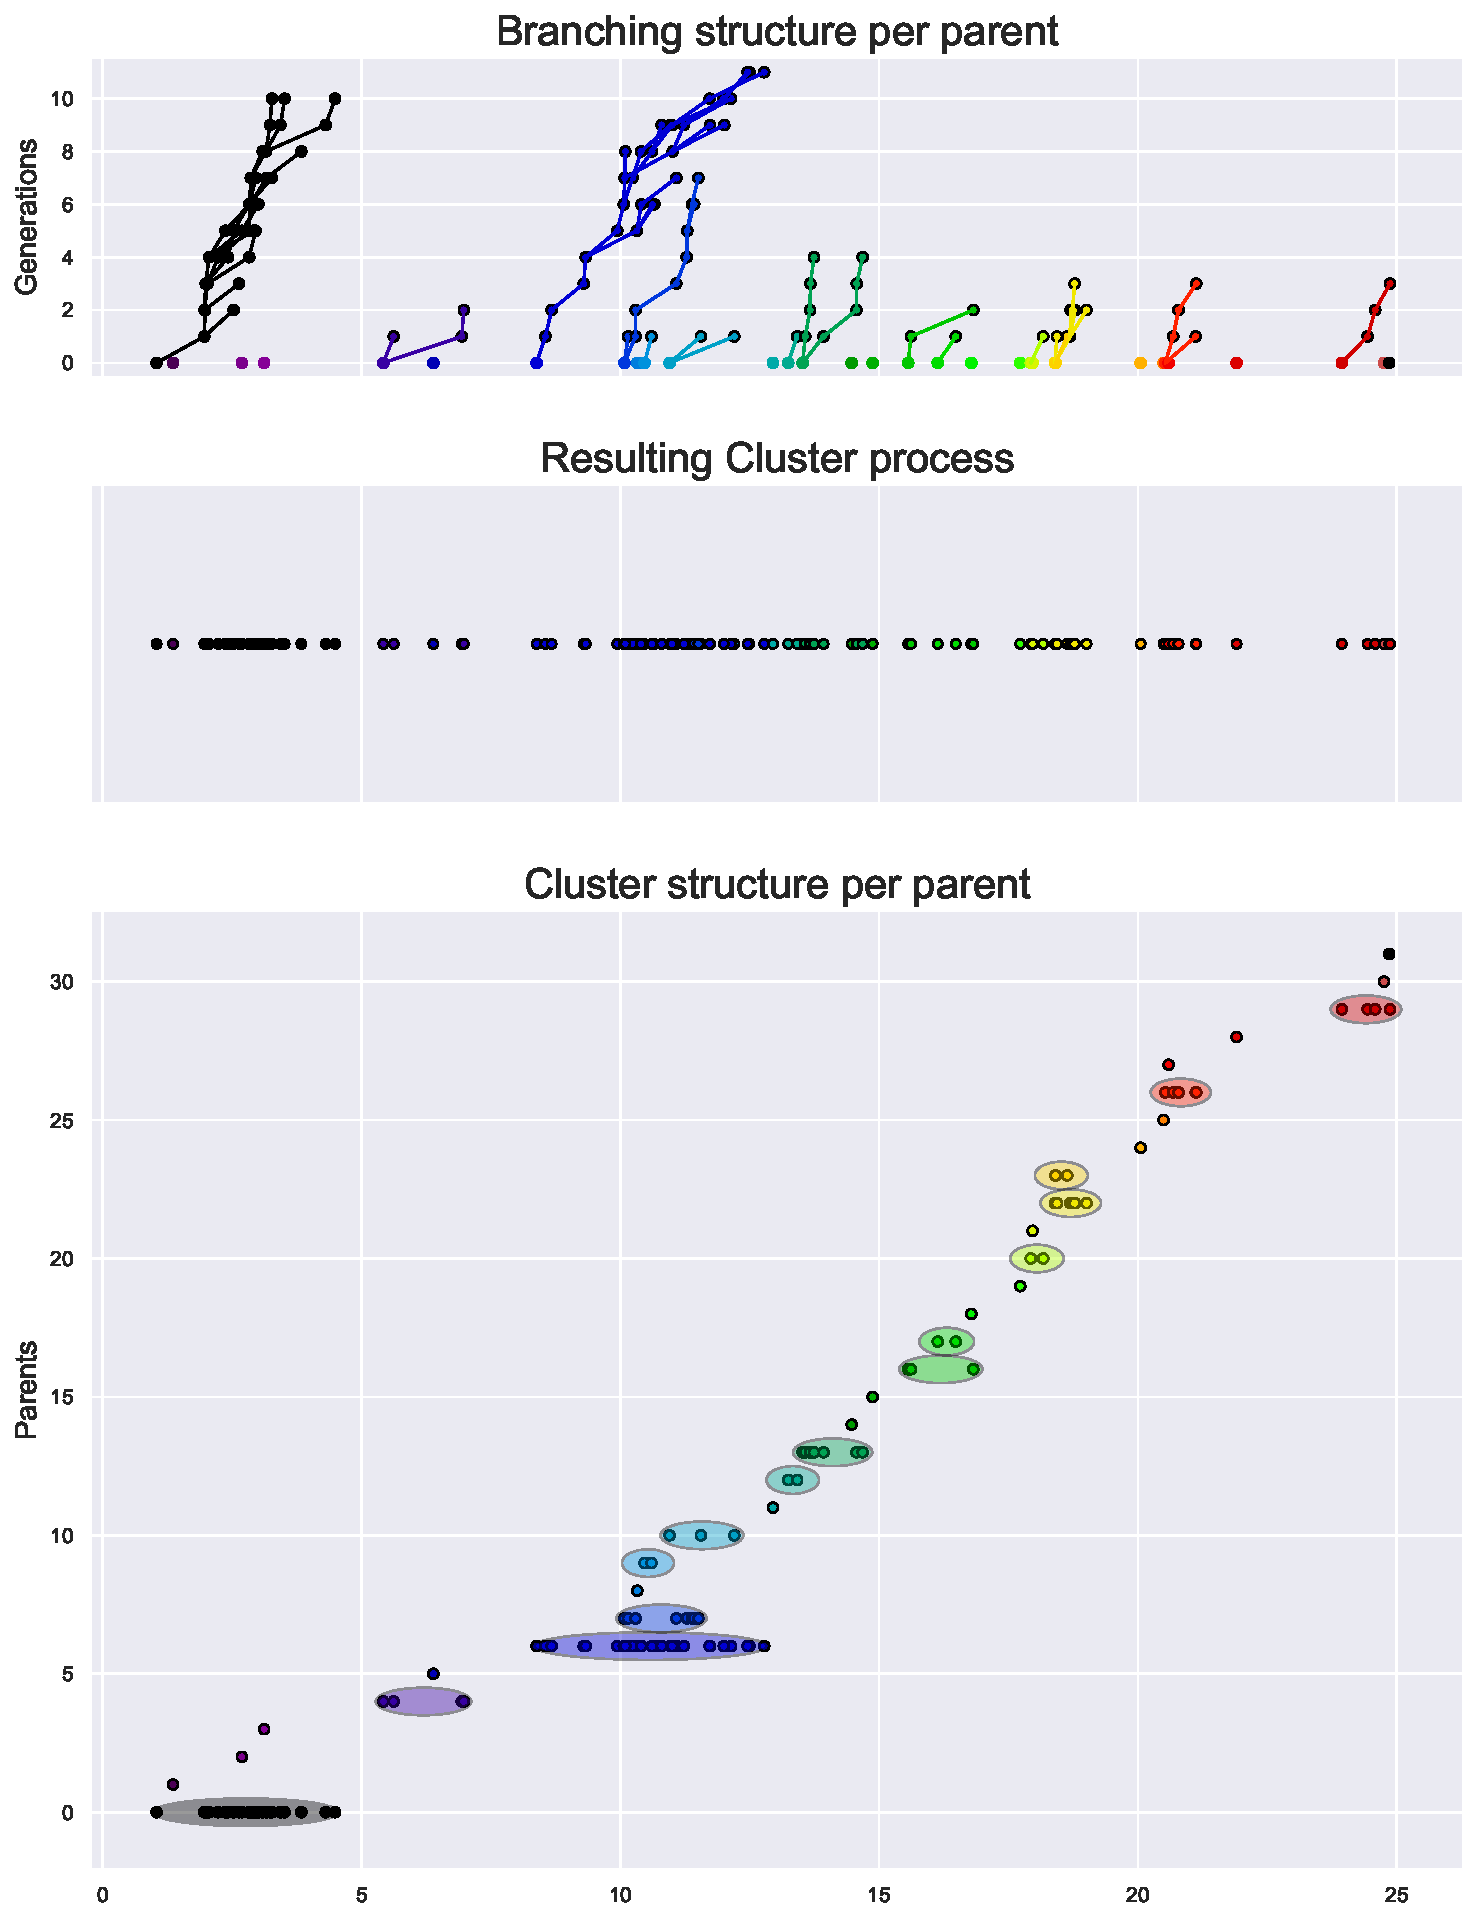
\includegraphics[width=0.95\textwidth]{images/chapter0/branching_and_cluster05.pdf}
      \caption{Illustration of both branching (top) and clustering (bottom) structures of an exponential Hawkes process (middle). Each color represents a single cluster/tree. Simulation is done thanks to the cluster process algorithm.
      }
      \label{fig:branching_and_cluster05}
    \end{figure}

    From a numerical point of view, the definition of a Poisson cluster process, as given above, provides a simulation algorithm. An inference method inspired from branching process theory was adapted to the study of Hawkes processes \parencite{Veen2008}.

    The aforementioned properties, and the quick developments that followed in the literature, created a growing interest in other scientific fields.
    From this, different versions of the original self-exciting Hawkes process appeared in the literature, each one trying to accommodate to more complex phenomena.

    \subsubsection{The multivariate Hawkes process} 
    Probably the most natural and useful extension is the definition of the \emph{multivariate} Hawkes process. 
    Instead of studying a single phenomenon (a univariate process), we define a $d$-variate Hawkes process as $d$ individual point processes $(N_i)_{i=1:d}$ interacting together, 
    where each process is defined by a conditional intensity function $\lambda^i$:
    \[\lambda^i(t) = \mu_i + \sum_{j=1}^{d}\sum_{T_k^j \leq t}{h_{ij}(t-T_k^j)}\,, \qquad \text{for any $t\in\RR$.}\]

    In this formulation, each process $N_j$ has its own event times $(T_k^j)_{k\in\ZZ}$ and baseline intensity $\mu_j > 0$.
    This model introduces interactions between processes, which appear in the second term of the intensity.
    The kernel functions $h_{ij}$ represent the effect of points from $N_j$ on process $N_i$.
    This model allows to study a group of individuals linked by a network of interactions, adding a new dimension of study for such processes.

    From modelling infection spread all the way to analysing clusters of earthquakes, the study of Hawkes processes from a statistical point of view quickly became a central topic of interest.

    \subsection{Inference and applications}

    \subsubsection{Statistical estimation}
    %Presenting an exhausting bibliography on statistical estimation for Hawkes processes would represent a titanical task, 
    %specially due to the numerous alternative models introduced since their introduction.
    %Nonetheless, we propose here a general overview of the estimation panorama in the literature for self-exciting Hawkes processes.
    
    Statistical challenges for Hawkes processes with excitation focus around estimating both the baseline intensity $\mu$ and the interaction function $h$.
    %In parametric settings, many kernel functions are traditionnally used (as some mentioned in the previous section),
    %each one defined by a parameter $\gamma\in\RR^m$ for a certain integer $m$.

    %\Add theta and statistical model

    To our knowledge, the very first paper implementing an estimation procedure in a parametric framework is \textcite{Adamopoulos1976}.
    In his work, the author proposes a study of exponential kernels for both univariate and bivariate Hawkes processes through the spectral log-likelihood,
    closely related to time series theory.
    The exponential kernel is often chosen as a parametric interaction function because in this case the univariate Hawkes process becomes a Markov process which presents the advantage of simplifying the expression of the intensity function. 
    This is exemplified in the implementation of the maximum likelihood estimator (MLE) in \textcite{Ozaki1979}.
    The expression of the log-likelihood of a general point process, for an observation in $[0, T]$, is:
    \begin{equation}\label{eq:chap0_loglikelihood}
      \ell_T(\theta) = - \int_{0}^{T}{\lambda(u)\,\dd u} + \sum_{k=1}^{N(T)}{\log(\lambda(T_k^-))}\,,
    \end{equation}
    where $N(T)$ is the number of points in the observation window. 
    Other works address estimation in the parametric setting, such as \textcite{Ogata1988} for other kernel functions using the MLE, \textcite{Veen2008} leveraging the branching structure, \textcite{Bacry2020} minimising a least-squares contrast and \textcite{DaFonseca2013} via the method of moments.

    The literature regarding non-parametric inference is also vast with implementations of the MLE in \textcite{Guo2018} and a penalised variant optimised by an Expectation-Maximisation algorithm.
    The least-squares minimisation is often used as shown in \textcite{Reynaud2010, Eichler2016, Kirchner2017}.
    Other methods include solving Wiener-Hopf equations \parencite{Bacry2016} or approximating the interaction functions with autoregressive models \parencite{Kirchner2017}.

    All of these references concern frequentist approaches of statistics, 
    and so it is essential to mention that an equal effort has been made from a Bayesian point of view.
    \textcite{Rasmussen2013} proposes two procedures through log-likelihood estimation: 
    one through the classical intensity function and another similar to \textcite{Veen2008} with the branching structure.
    In \textcite{Lemonnier2014}, the authors propose an approximation through exponential kernels and taking advantage of the Markovian properties.
    The multivariate case is deeply studied in \textcite{Donnet2020} with illustrations on estimating the underlying interaction graph.
    
    This is jus a small sample of the plethora of approaches that have been developed in order to study these kind of processes.
    
    \subsubsection{Applications and generalisations}
    % The main motivation behind the works presented in this thesis, as it has been and continues to be for researches in this field,
    % is to use the versatility of the model and its exceptional adaptability to propose new submodels.
    % When confronted to real-world data, 
    % researchers tend to reformulate and complexify the Hawkes model in order to better describe the studied phenomena. 
    The temporal-dependency structure of Hawkes process has motivated its use accross a variety of application fields with many generalisations to obtain more explicative models.

    The historical example is the study of seismic activity where the occurrence of an earthquake is usually followed by a number of smaller tremors known as aftershocks.
    This behaviour is similar to the self-exciting effect modelled by the Hawkes process and associated with the clustering structure, as shown in \textcite{Adamopoulos1976}.
    As in seismology the spatial placement and magnitude of each quake are important factors to take into account, applications in this field tend to include this information via the concept of marked point processes. 
    Each event time has an associated mark representing the detected magnitude \parencite{Ogata1988} and the location of each epicenter \parencite{Ogata1998, Kwon2023}.
    %Further develop

    A similar approach is proposed in the study of social media interactions for the analysis of subject trends.
    The excitation effect appears in the form of reposting where users have the option to share a news post among their followers which in turn may continue to spread the information in their social circles.
    In this context, the impact of each repost is dependent on the influence of the account and the impact of a topic on a certain community.
    This is represented for example by including information in the form of number of followers \parencite{Mishra2016} again through marks, or by adding an additional dimension to the process \parencite{Pinto2015} to represent the impact of a topic over another.

    In criminology, it is commonly assumed that delinquent acts may incite other crimes in a population, which can be modelled by a self-exciting Hawkes process.
    As a branch of social sciences, it is important to account for different factors that affect human behaviour such as time of the day, demographics and social interactions.
    A way of accounting for these effects is to adapt the Hawkes process to time and spatial dependent baseline intensities. 
    A time-varying baseline intensity can represent periodic criminal behaviour \parencite{Lewis2011} with higher values for nightime.
    A space-dependent baseline is used to represent the link between residential density and burglary \parencite{Mohler2011} or the spatial distributions of gangs in a city \parencite{Linderman2014}.

    % Working in high dimensions allows to account for high number of individuals with sparse networks of interactions.
    % Penalisation methods in the study of neuronal spike trains \parencite{Reynaud2013, Lambert2018}
    % allow to reduce the support (non-null interactions) of the connectivity matrix.
    % This allows to improve estimations, allow for better computational times and more importantly provide more explicative models for the experts.

    Many other fields include finance \parencite{Embrechts2011, Bacry2013, Roueff2019, Lotz2024}, genomics \parencite{Reynaud2010, Carstensen2010}, ecology \parencite{Denis2024, Nicvert2024}, epidemiology \parencite{Rizoiu2018, Chiang2022}, TV browsing behaviour \parencite{Xu2016}, event data streams in football \parencite{Baouan2023, Narayanan2023}, 
    each one often accompanied with new formulations of the Hawkes process.

    \subsection{Challenges and contributions}

    Our work is motivated by the applications of Hawkes processes in neurobiology for the study of neuronal activity data \parencite{Reynaud2013, Lambert2018, Duval2021}.
    Neurons in the brain are connected through a deep network of synapses allowing them to communicate through electrical impulses usually studied by measuring the action potential or spikes emitted as the membrane potential of the cells is depolarised.
    These measurements generate a spike train of instants when a neuron activates and influences the membrane potential of connecting neighbours.

    These exchanges can appear either as excitatory or inhibitory to respectively incite or stop other neurons from activating.
    The first effect can be clearly modelled by a multivariate Hawkes process but the original modelling does not account for inhibiting effects.
    In practice, this requires to allow for the interaction functions $h_{ij}$ to take negative values, introducing the concept of Hawkes processes with inhibition.

    In order to guarantee the non-negativity of the intensity function, a common practice in the literature is to consider the concept of \emph{non-linear Hawkes processes}.
    The main difficulty is that the branching structure of Hawkes processes is not valid any longer and the intensity function presents more complex behaviour, so pre-established inference methods are not accessible anymore.
    The first part of this manuscript pertains to the study of inhibiting Hawkes processes in order to propose estimation methods in the parametric setting.
    We present an overview of the studied model and our contributions in Section~\ref{sec:chap0_inhibition}.
    
    The second part of this manuscript is focused around studying imperfect data.
    Collecting spike trains data is a procedure that can present measurement errors, which can appear as missing neuronal activation instants or by attributing spikes to the wrong neuron.

    This setting represents a common statistical framework of accounting for missing data in an observed process.
    In our context, not having a full knowledge on the past history of the process makes the conditional intensity function intractable.
    Our contributions, as summarised in Section~\ref{sec:chap0_missing_data}, are focused on exhibiting an inference paradigm through the spectral analysis of point processes for observations noised either by adding points from an external process or by deleting event times. 

    Although the models inbetween chapters may differ, our contributions follow a common thread by addressing the following four questions.
    \vspace{5mm}
    \begin{tcolorbox}
      \begin{itemize}
        \item What approaches can we take to establish parametric estimation procedures for more complex Hawkes processes dynamics?
        \item Under which conditions are our statistical models identifiable?
        \item How to evaluate and select the best estimators through data-driven methods?
        \item Which modern statistical tools can we leverage to improve our inference procedures?
      \end{itemize}
    \end{tcolorbox}
    
    %These questions may serve as a general guide when reading this manuscript.

    %\subsection{Questions} %and contributions}
    % \begin{itemize}
    %     %\item In this thesis we study two extensions: 
    %     %\item In the first half (chapters) we study inhibition 
    %     %\item In the second half (chapters) we study missing data.
    %     \item Our studies are articulated along 3 general questions (i) what approaches for considering alternative or more complex dynamics than self-excitation in parametric and what properties can we establish; (ii) how to evaluate and select our models through data-based methods in multivariate cases (null interactions); (iii) what statistical tools allow us to improve inference.
    % \end{itemize}

% mentionner faire des outils accessible, partage du code (open source, facilité)
% mettre/valoriser les codes ici 

\section{Factoring in inhibition for Hawkes processes}\label{sec:chap0_inhibition}
    
    \subsection{Context and related works}
    The original Hawkes process was proposed as a way of modelling the effect of excitation between points, which is characterised by the positivity of the interaction function $h$.
    Our first goal in this work is to study the opposite effect which is commonly known in the literature as \emph{inhibition}.
    
    An inhibiting Hawkes process consists in modelling repulsion between points: each event will reduce the chances of others occurring during a certain period of time.
    Mathematically, a way of translating this effect is by allowing $h$ to take negative values. However, the non-negativity condition on $\lambda$ prevents us from adopting this approach without adding some constraints.

    One of the most common solutions is the \emph{non-linear} Hawkes process model. In the univariate setting, let $h:\RR_{\geq 0} \to \RR$ and $\Phi:\RR\to\RR_{\geq 0}$ be two measurable functions. We define a univariate non-linear Hawkes process $N$ on the real half-line $\RR_{\geq 0}$ with event times $(T_k)_{k\in\NN}$ by the conditional intensity function, for any $t\in\RR_{\geq 0}$:
    \begin{equation}\label{eq:chap0_nonlinear_intensity}
      \lambda(t) = \Phi\left(\mu + \sum_{T_k \leq t}{h(t-T_k)}\right)\,.
    \end{equation}
    By allowing $h$ to be negative, the function $\Phi$ has to be a non-linear function. Existence of such processes is ensured as long as $\Phi$ is an $L$-Lipschitz function \parencite[Theorem 1]{Bremaud1996} such that:
    \[L\int_{0}^{+\infty}{\lvert h(t)\rvert\,\dd t} <1\,.\]
    Multiple choices exist in the literature like a clipped exponential function \parencite{Chornoboy1988,Carstensen2010,Gerhard2017}, a softplus function \parencite{Mei2017}, a sigmoid function \parencite{Menon2018}, among others.
    
    In our work, we choose the positive part (ReLU) $\Phi(\cdot) = (\cdot)^+ = \max(0, \cdot)$ like in \textcite{Lemonnier2014, Hansen2015, Lu2018, Costa2020}.
    The intensity function (Equation~\eqref{eq:chap0_nonlinear_intensity}) becomes:
    \begin{equation}\label{eq:chap0_nonlinear_univariate_intensity}
      \lambda(t) = \left(\mu + \sum_{T_k \leq t}{h(t-T_k)}\right)^+\,,
    \end{equation}
    and the extension to a $d$-variate Hawkes process is:
    \begin{equation}\label{eq:chap0_nonlinear_multivariate_intensity}
      \lambda^i(t) = \left(\mu_i + \sum_{j=1}^{d}\sum_{T_k^j \leq t}{h_{ij}(t-T_k^j)}\right)^+\,,
    \end{equation}
    for each process $N_i$.

    Our general contribution in the context of Hawkes processes with inhibition is to provide parametric estimation procedures in a frequentist framework through maximum likelihood estimation.
    To our knowledge, and by the time of publication of both corresponding papers, other frequentist approaches \parencite{Reynaud2014,Bacry2016} do not model inhibition but can provide negative estimations.
    In Bayesian contexts, works modelling non-linear Hawkes processes focus around the log-likelihood. In \textcite{Deutsch2022}, the compensator is computed exactly in the case where the interaction functions $h_{ij}$ are exponential with shared decay rate (a similar result to the one presented in Chapter~\ref{chapter:multivariate_inhibition}, obtained independently
    during the same period). In practice, an approximation of the compensator through a Simpson's rule is proposed for more general scenarios. This gives access to posterior density estimates in a parametric setting. %In parenthesis cite and then approximation in practice
    Works in non-parametric settings include \textcite{Sulem2024} that derives posterior concentration rates and \textcite{Sulem2023} proposing a variational Bayes method and a sparsity-inducing version based on a model selection paradigm.

    \subsection{Maximum Likelihood Estimation for Hawkes Processes with self-excitation or inhibition}
    
    In Chapter~\ref{chapter:univariate_inhibition}, we focus on the study of the univariate Hawkes process $N$ with intensity function described by Equation~\eqref{eq:chap0_nonlinear_univariate_intensity}.
    In order to establish the maximum likelihood estimator for a parametrised model of the intensity with parameter $\theta\in\Theta$, 
    it is necessary to obtain a closed-form expression of the log-likelihood:
    \[\ell_T(\theta) = - \int_{0}^{T}{\lambda_\theta(u)\,\dd u} + \sum_{k=1}^{N(T)}{\log(\lambda_\theta(T_k^-))}\,.\]
    
    For Hawkes processes with excitation, the linearity of the intensity function results in an explicit expression of $\ell_T$ without much trouble, as shown in \textcite{Ozaki1979}.
    The main difficulty when including inhibition is that the cumulated effects from the past events may saturate process $N$, meaning that its intensity is null for a certain period of time.
    In the work of \textcite{Lemonnier2014}, the authors propose to approximate the computation in this context by ignoring the non-linear function.
    This allows them to circumvent this problem at the cost of assuming that the inhibition effects are small enough to be negligible.

    In order for us to obtain an exact computation of the log-likelihood that accounts for inhibition, we introduce two novel concepts: the \emph{underlying} intensity function $\lambda^\star$ and the \emph{restart times} $(T_k^\star)_{k\geq 1}$.
    We define $\lambda^\star\colon \RR_{\geq 0}\to \RR$, for any $t\geq 0$, as:
    \[\lambda^\star(t) = \mu + \sum_{T_k \leq t}{h(t-T_k)}\,,\]
    and the restart times $T_k^\star$ for any integer $k>0$ as:
    \[T_k^\star = \inf\{t\geq T_k \mid \lambda(t) > 0\}\,.\]

    The advantage of working with $\lambda^\star$ instead of $\lambda$ is that it inherits properties such as smoothness and strict monotonicity from the interaction function $h$ between any two consecutive event times $T_k$ and $T_{k+1}$.
    If assumed so, it follows that $T_k^\star$ is the moment from which both functions coincide.
    Our main contribution is to provide a closed-form expression of the compensator $\int_{0}^{T}{\lambda_\theta(u)\,\dd u}$, which we establish in Proposition~\ref{prop:chap0_integral_cooldown}.
    \begin{proposition}\label{prop:chap0_integral_cooldown}
      For any $t>0$:
      
      \begin{equation}\label{eq:chap0_compensator_general}
      \int_{0}^{t}{\lambda(u)\,\dd u} =
      \begin{dcases}
          \mu t &\text{\qquad if $t<T_1$}\\
          \mu T_1 + \sum_{k=1}^{{N(t)-1}}{\int_{T_{k}^\star}^{T_{k+1}}{\lambda^\star(u)\,\mathrm{d}u}} + \int_{T_{N(t)}^\star}^{t}{\lambda^\star(u)\,\mathrm{d}u} &\text{\qquad if $t\geq T_1$}\,,
      \end{dcases}
      \end{equation}
      with the conventions that the sum is equal to $0$ if ${N(t)} = 1$ and the last integral is equal to $0$ if $t < T_{N(t)}^*$.

      If we consider the exponential kernel $h\colon t\mapsto \alpha \mathrm{e}^{-\beta t}$ for parameters $\alpha > 0$, $\beta > 0$, then the restart times read:
      \[
          T_k^\star = T_k + \beta^{-1} \log \left({\frac{\lambda_0 - \lambda^\star(T_k)}{\lambda_0}} \right) \II_{\lambda^\star(T_k) < 0}\,,
      \]
      and, for any integer $k\geq 1$ and any $\tau \in [T_{k}^*, T_{k+1}]$, each integral simplifies to 
      :
      \[
          \int_{T_{k}^\star}^{\tau}{\lambda^\star(u)\,\mathrm{d}u}
          = \lambda_0(\tau - T_{k}^\star) + \beta^{-1} (\lambda^\star(T_{k}) - \lambda_0) (\mathrm{e}^{-\beta(T_{k}^\star-T_{k})}-\mathrm{e}^{-\beta(\tau-T_{k})})\,.
      \]
      \end{proposition}

    This result allows to establish the maximum likelihood estimation procedure that accounts for both self-exciting and self-inhibiting effects, while keeping the same computational complexity as the method implemented in previous works. 
    In particular, for the exponential kernel function, the computational complexity of $\ell_T$ is $O(N(T))$ thanks to the Markovian property and, as shown in our numerical study, the derived estimations are better than by using an approximation framework (as presented in \textcite{Lemonnier2014}) especially for high levels of inhibition effects.

    A second consequence of Proposition~\ref{prop:chap0_integral_cooldown} is that it gives access to a goodness-of-fit measure for our estimations by leveraging the Time Change theorem of point processes \parencite[Theorem 7.4.IV]{DaleyV1}.
    In particular, this allows us to introduce a hypothesis testing procedure that evaluates the quality of our estimations on an independent set of observations.
    
    % With this result, it suffices to obtain a closed-form expression of the restart times, which we explicit in the case of the exponential kernel function.
    % We define then the maximum likelihood estimation procedure through an iterative algorithm to compute $\ell_T$.
    % An outstanding property of our approach is that it allows to account for both self-exciting and self-inhibiting effects, without increasing the computational complexity.

    % Our numerical study illustrates the efficiency of our estimator in multiple scenarios.
    % As expected, we demonstrate the importance of correctly accounting for inhibition in our estimation procedure. When compared to the approximation framework in \textcite{Lemonnier2014}, 
    % our approach provides better estimates in the exponential context, specially when the inhibition effects are consequential.
    % Finally, as a consequence of Proposition~\ref{prop:chap0_integral_cooldown}, we are able to implement a goodness-of-fit assessment of our models through the Time Change theorem of point processes \parencite[Theorem 7.4.IV]{DaleyV1}.
    % This allows to introduce a hypthesis testing procedure that allows to evaluate the quality of our estimations on an independent set of observations.





    \subsection{Inference of multivariate exponential Hawkes processes with inhibition and application to neuronal activity}
    Chapter~\ref{chapter:multivariate_inhibition} builds upon the bases established in Chapter~\ref{chapter:univariate_inhibition} to derive an estimation procedure for multivariate Hawkes processes $N = (N_1, \ldots, N_d)$. 
    In this setting the log-likelihood of $N$ reads:
    \[\ell_T(\theta) = \sum_{i=1}^{d}{\left(- \int_{0}^{T}{\lambda_\theta^i(u)\,\dd u} + \sum_{k=1}^{N_i(T)}{\log(\lambda^i_\theta(T_k^{i-}))} \right)}\,,\]
    where $\lambda^i_\theta$ and $(T_k^i)_k$ are respectively the candidate intensity and event times of $N_i$.
    Process $N$ can be seen as a univariate point process with its event times $(T_{(k)})_k$ being the ordered union of $(T_k^i)_k$ for all integers $i=\{1, \ldots, d\}$.
    To alleviate the notations, we will omit the subscript $\theta$ unless said otherwise.
    Similarly to the univariate case, we propose to study the underlying intensity functions $\lambda^{i\star}$:
    \[\lambda^{i\star}(t) = \mu_i + \sum_{j=1}^{d}\sum_{T_k^j \leq t}{h_{ij}(t-T_k^j)}\,,\]
    but this time the monotonicity condition of $h_{ij}$ is not enough to retrieve useful properties for this functions.

    This is a consequence of the increased complexity of the dynamics of each subprocess that allows both exciting and inhibiting effects to exist simultaneously.
    In the multivariate setting, it is possible for a subprocess $N_i$ to be saturated ($\lambda^i(t)=0$) at an instant $t$ and to receive an external excitation of another subprocess.
    So, in order to simplify our problem, we restrict our study to the exponential kernel case $h_{ij}(t) = \alpha_{ij}\mathrm{e}^{-\beta_{ij} t}$ with the following mild assumption.

    \begin{assumption}\label{assu:chap0_beta}
      For each $i\in\{1,\ldots, d\}$, there exists $\beta_i\in\RR_{>0}$ such that $\beta_{ij} = \beta_i$ for all $j\in\{1,\ldots, d\}$.
    \end{assumption}
    This allows us to recover the strict monotony of $\lambda^{i\star}$ between any two event times $T_{(k)}$ and $T_{(k+1)}$ of the general process $N$.
    With this, we adapt the expression of the restart times $(T_{(k)}^{i\star})_{k\geq 1}$ and the compensator $\int_{0}^{t}{\lambda^i(u)\,\mathrm{d}u}$ for each process $N_i$ and every event time $T_{(k)}$, allowing us to establish our first contribution in the form of Proposition~\ref{prop:chap0_compensator}.

    \begin{proposition}\label{prop:chap0_compensator}
      Let us suppose that Assumption~\ref{assu:chap0_beta} is granted. 
      Then, for each $i\in\{1,\ldots, d\}$ and any $k\geq1$, we have:
      
      \begin{equation}\label{eq:chap0_restart_times_exponential}
        T\park^{i\star} = \min{\adaptedpar{t^\star_k, T\park[k+1]}}\,.
      \end{equation}
      where
      \[t^\star_k = \adaptedpar{T\park + \beta_i^{-1}\log{\adaptedpar{\frac{\mu_i - \lambda^{i\star}(T\park)}{\mu_i}}}\II_{\{\lambda^{i\star}(T\park) < 0\}}}\,.\]
      And, for each $i\in\{1,\ldots, d\}$, the compensator of the process $N_i$ reads, for any $t\geq 0$:
      \begin{equation}\label{eq:chap0_compensator_exponential}
        \int_{0}^{t}{\lambda^i(u)\,\mathrm{d}u} =
        \begin{cases}
          \mu_i t & \text{if } t < T\park[1] \\
          \mu_i T\park[1] + \sum_{k=1}^{N(t)} J_k & \text{if } t \geq T\park[1] \,,
        \end{cases}
      \end{equation}
      where for all integer \(k \in \{1, \dots, N(t)\}\):
      \begin{equation*}
        J_k =
        \mu_i \left[\min(t, T\park[k+1] ) - T\park^{i\star}\right] + \beta_i^{-1} \left(\lambda^{i\star}(T\park) - \mu_i \right)
        \left[ \mathrm{e}^{-\beta_i(T\park^{i\star} - T\park)} - \mathrm{e}^{-\beta_i(\min(t, T\park[k+1])- T\park)} \right]\,.
      \end{equation*}
      \end{proposition}

      With this result, we establish an exact procedure to compute the log-likelihood $\ell_T^i$ of each process $N_i$, giving us access to the complete log-likelihood $\ell_T$ and in turn, access to the maximum likelihood estimation method.
      Let us note that as in the univariate case, we also get access to a goodness-of-fit procedure via the Time Change theorem.
      
      Another complication in the multivariate setting is that the identifiability of our statistical model for the exponential Hawkes process is not as straightforward as in the univariate case. 
      To partially answer this question, we provide a sufficient condition in Theorem~\ref{th:chap0_identifiability} to ensure the identifiability of the intensity functions.

      \begin{theorem}[Identifiability]\label{th:chap0_identifiability}
        For all $i\in\{1, \ldots, d\}$, let $\theta_i \in \Theta$ be a parameter for $\lambda^i$.

        Let us assume that a.s.\ for every $(i, j) \in \{1, \dots, d\}^2$, $i\neq j$,
        there exist an event time \(\tau\) from process \(N_j\),
        and an event time \(\tau_+ > \tau\) from process \(N_i\), such that:
        \begin{enumerate}
            \item $\lambda_{\theta_i}^i(\tau^-) > 0$;
            \item there are only events of process $N^j$ in the interval $[\tau, \tau_+)$.
        \end{enumerate} 
        
        Then,
        \[
          \forall i \in \{1, \dots, d\},~
          \lambda_{\theta_i}^i(t) = \lambda_{\theta_i'}^i(t) \text{ a.e.}
          \qquad
          \iff
          \qquad
          \forall i \in \{1, \dots, d\},~\theta_i = \theta'_i\,.
        \]
    \end{theorem}

      Overall, this condition allows to avoid pathological situations either when some process $N_i$ is not observed (strong external inhibition effects), or when there is a cyclical observation of points (strong internal inhibition effects).

      Finally, we present a solution for estimating the interaction network of a multivariate Hawkes process.
      As it is common in real-data contexts, it is often unrealistic to assume that all functions $h_{ij}$ are non-null, meaning that all processes interact with each other.
      For this, we propose three different data-driven techniques based on a thresholding approach inspired by principal component analysis, and based on the construction of confidence intervals (Student and empirical).
      Our results on synthetic data show a significant improvement with respect to other state-of-the-art methods \parencite{Lemonnier2014, Bacry2020}.
      In particular, when the interaction matrix $(\alpha_{ij})_{i,j=1:d}$ contains null entries, we implement our post-hoc procedures to obtain an estimation of the connectivity network before re-estimating all non-null entries on a reduced model.
      This provides the best estimations, in the sense of the $\ell_2$ relative error, among the considered models, as confirmed by our results on real-data concerning the analysis of neuronal activity.



\section{Something is amiss: spectral methods for imperfect data}\label{sec:chap0_missing_data}
    
  \subsection{Context and related works}
  In the second part of the thesis, we turn the spotlight to a common issue in statistics: 
  establishing efficient estimation procedures when the observed data is noised in some sense.

  In the context of point processes, a natural approach to define noised models is through the operations of thinning, superposition and jittering.
  \begin{enumerate}
    \item The \textbf{superposition} of two point processes $X$ and $Y$, usually noted $X+Y$ is the point process defined by the ordered union of event times $(T_k^X)_k$ and $(T_k^Y)_k$.
    \item The \textbf{thinning} of a point process $X$ corresponds to erasing some event times $T_k^X$ through a random rule.
    When point are erased independently from each other with a common probability $1-p$, we talk about a $p$-thinning of process $X$.
    \item The \textbf{jittering} of a point process consists in the random displacement of points.
  \end{enumerate}

  The main interest of studying such alterations is to account for various measurement errors in real-world data. 
  The most commonly studied in the literature is jittering which tends to appear when spatial imprecisions add a layer of uncertainty. 
  Literature tends to focus on Poisson processes \parencite{Antoniadis2006, Hohage2016, Bonnet2022},
  with Hawkes processes being studied in \textcite{Trouleau2019, Deutsch2020}.

  Thinning is often used to represent missing data but has been scarcely studied in the literature. \textcite{Mei2019} propose a method to complete a sequence of times that have missing points via a Long Short-Term Memory neural network model based on the Hawkes process.
  
  The study of superposition allows to account for observations that are contaminated by points originated from an external process, but are indistinguishable from those of the original process. 
  To our knowledge, the only work that studies this kind of noise is \textcite{Lund2000}, which in fact tackles a general point process that is potentially noised by the three aforementioned mechanisms.
  Their work establishes an approach by maximising the conditional log-likelihood dependent on the original process with an application to Hawkes processes.
  In practice and for numerical reasons, they propose a local maximiser of this quantity in a small set of parameters when having access to an estimation of the unnoised process.

  Other imperfect data models have been presented in \textcite{Linderman2014} where the authors favour a Bayesian approach through latent variables to study processes with missing marks, unobserved time intervals or unobserved subprocesses. 
  The last work we mention here is \textcite{Cheysson2022}, where the exact locations of the points of a Hawkes process are not known. 
  Instead, the only information available is the number of points that fall inside equally-sized intervals.
  They leverage then the spectral theory of point processes and time series in order to provide an estimation procedure that does not necessitate the precise location of event times.
  
  Our contribution is to make use of the spectral theory of point processes, centered around the Bartlett spectrum \parencite{Bartlett1964} and the Whittle estimator \parencite{Whittle1952}, in order to propose estimators for Hawkes processes altered by superposition (Chapter~\ref{chapter:spectral_superposition}) and thinning (Chapter~\ref{chapter:spectral_thinning}).
  Another contribution is to leverage the obtained inference method to incorporate a subsampling paradigm through thinning for small observation windows.
  The existing spectral theory for Hawkes processes is limited to exciting interactions, so we restrict our models to this framework.
  
  
    %\begin{itemize}
    %    \item Introduce the point process operations and provide missing data formalism. 
    %    \item Bibliography
    %\end{itemize}




    \subsection{Spectral analysis for the inference of noisy Hawkes processes}
    Chapter~\ref{chapter:spectral_superposition} is dedicated to the study of the superposition of a Hawkes process $H$ with exciting kernel functions and an independent homogeneous Poisson process $P$ with intensity $\lambda_0 > 0$.
    We consider their superposition, that we note $N = H + P$,
    and we assume that we have no knowledge on the origin of each event time $T_k^N$ (either Hawkes or Poisson).
    The intensity function of this resulting process is intractable and any method based on it is therefore inaccessible. 
    
    As mentioned previously, we take inspiration from \textcite{Cheysson2022} in order to leverage the spectral approach of point processes to circumvent this issue. 
    The Bartlett spectrum $\Gamma^N$ of $N$ is a measure defined by the means of the Fourier transform of its reduced covariance measure.
    When this measure is absolutely continuous, its density is noted $f^N$ and often called the spectral density of the process.
    We can establish an estimation procedure of a parametric model for $f^N$ (with parameter $\theta\in\Theta$) through the periodogram function $I^T$.
    For an observation $(T_k^N)_{k\geq 1}$ in $[0,T]$, the periodogram is defined, for any $\omega\in\RR$, as:
    \begin{equation}\label{eq:chap0_periodogram}
      I^T(\omega) = \frac{1}{T}\sum_{k=1}^{N(T)}\sum_{l=1}^{N(T)}{\mathrm{e}^{-2\pi \iu \omega (T_k^N - T_l^N)}}\,.
    \end{equation}
    Asymptotically, this quantity follows an exponential distribution with mean $f^N(\omega)$ and so it is possible to define the maximum spectral log-likelihood estimator $\hat \theta$ as:
    \begin{equation}\label{eq:chap0_spectral_estimator}
      \hat \theta \in {\arg\max}_{\theta\in\Theta} %\left(
        -\frac{1}{T}\sum_{k=1}^{M}{\left(\log\left(f_\theta^N(\omega_k)\right) + \frac{I^T(\omega_k)}{f_\theta^N(\omega_k)}\right)}%\right)
        \,,
    \end{equation}
    where $\omega_k = k/T$ for $k\in\{1,\ldots,M\}$.
    What makes this quantity so useful in our context is that it can be exactly computed without any information on the source of event times $(T_k^N)_k$. 

    Our first result establishes the expression of the spectral density function for the superposition of two independent point processes as exhibited in Proposition~\ref{prop:chap0_sum_of_spectral_densities}.

    \begin{proposition}\label{prop:chap0_sum_of_spectral_densities}
      Let $X$ and $Y$ be two independent and stationary point processes, admitting respective spectral densities ${f}^X$ and ${f}^Y$.
      
      Then $N = X + Y$ admits a spectral density function $f^N$ and
      \begin{equation} \label{eq:chap0_sum_spectral_densities}
        {f}^N = {f}^X + {f}^Y\,.
      \end{equation}
    \end{proposition}
    As the spectral density of a Hawkes process is explicit \parencite[Example 8.2(e)]{DaleyV1}, we obtain the general form of the spectral density of our noisy Hawkes process, which in turn makes it possible to establish an estimation procedure by maximising the spectral log-likelihood.

    %To correctly work with these tools, it is necessary to consider stationary point processes,
    %which for the case of Hawkes processes necessitates to consider processes in the entire real line $\RR$.
    
    Our main contribution in the univariate setting is to establish conditions for the identifiability of $f^N$ for different parametrisations of the kernel function $h$. 
    The first result is related to the classical exponential kernel. 
    We show that the model is identifiable if and only if one of the four parameters (three for the Hawkes process and one for the Poisson process) is fixed, even though the distribution of $N$ is uniquely determined without this constraint.
    Furthermore, we prove that the noisy Hawkes process with a uniform kernel function defines an identifiable spectral model.
    %We also prove that the noisy Hawkes process with an uniform kernel function defines an identifiable spectral model, which suggests that the non-identifiability issues is not  the spectral approach.
    %The non-identifiability derives then from the spectral approach and not from the superposition operation, as for a noisy Hawkes process with uniform interaction functions the model is identifiable
    %In order to determine whether the non-identifiability is due to the spectral approach or not, we study the noisy Hawkes process with uniform kernel and show that the spectral model is identifiable

    In the multivariate case, all tools from spectral theory exist and results are easily extended concerning the estimation procedure.
    Our contributions specifically concern the bivariate exponential Hawkes process noised by a bivariate Poisson process with common parameter $\lambda_0$.
    We present sufficient conditions on the interaction matrix $(\alpha_{ij})_{1 \leq i,j \leq 2}$ that characterise either the identifiability or non-identifiability of the corresponding statistical model.

    Our work is concluded by a numerical study in both the univariate and bivariate cases when identifiability conditions are verified.
    We show in both cases that our estimators perform particularly well, especially for processes with strong excitation effects and as the observation horizon $T$ increases.
    Our final contribution is to propose an ad-hoc procedure in the bivariate case that allows to determine the support of the interaction matrix by considering the empirical 5$\%$ quantiles of a sample of estimations, which in turn enhances the performance of our methods.
    




    \subsection{A numerical exploration of thinned Hawkes processes through spectral theory}
    Finally, Chapter~\ref{chapter:spectral_thinning} turns to the analysis of thinning for point processes.
    Let $H_p$ be a process issued from thinning a univariate Hawkes process with a probability $1-p$ of erasing each point $T_k$, for $k\in\ZZ$.
    As previously mentioned, any method based on the conditional intensity function is unavailable, so we turn to spectral theory.

    All the tools presented in the previous subsection can still be implemented here, in particular the expression of the periodogram (Equation~\eqref{eq:chap0_periodogram}) remains unchanged. 
    As a consequence, it can still be exactly computed even though we do not observe all points of the original process.
    In order to implement an inference procedure as defined by Equation~\eqref{eq:chap0_spectral_estimator}, we need to obtain an expression of the $p$-thinned process $H_p$.
    This is presented in Proposition~\ref{prop:chap0_spectral_thinning}.

    \begin{proposition}\label{prop:chap0_spectral_thinning}
      Let $H$ be a stationary point process admitting a spectral density function $f^H$ and let $m_1=\EE[\lambda(0)]$ be its average intensity.
      For any $p\in(0,1]$, let $H_p$ be a $p$-thinning of $H$.
  
      Then, $H_p$ admits a spectral density function, denoted $f^{H_p}$, such that for any $\omega\in\RR$:
      \begin{equation}\label{eq:chap0_spectral_thinning}
          f^{H_p}(\omega) = p^2 f^H(\omega) + p(1-p)m_1\,.
      \end{equation}
  
  \end{proposition}
    This result is obtained by leveraging the spectral theory of marked point processes as presented in \textcite{Bremaud2005}.

    We focus our study on the exponential kernel function and we prove that the derived statistical model is identifiable if and only if one parameter is fixed, similar to the aforementioned superposition scenario.
    We present numerical results under this condition by fixing the value of the thinning parameter $p$. 
    In particular, we show that our estimation method is robust with respect to the level of thinning, with remarkable results when enough event times are available for inference.
    %This is particularly encouraging, as the thinning procedure can dilute the interactions between the original points from process $H$.
    
    Our last contribution in this work is to make use of the thinning operation as a subsampling procedure when a single observation of $H$ is available in a small window of time.
    The use of subsampling for point processes has been done previously in the literature \parencite{Moller2003, Cronie2024} in order to improve estimation procedures.
    In our case, we focus on enhancing the quality of our spectral estimations by combining an $\ell_2$ penalisation with an averaged estimator obtained by thinning the unique observation of $H$.
    We show that our proposed procedure provides in general the best estimations, in the sense of the relative $\ell_2$ error, when compared to another subsampling procedure and displays a substantial improvement by reducing the high bias observed for the non-penalised estimator.
    
\section{Outline of the manuscript}\label{sec:chap0_outline}

    % This manuscript is divided in two parts, with Chapter~\ref{chapter:background} presenting a succinct presentation of point processes theory, from a random measure approach, and the formalism of Hawkes processes.
    % Let us note that all chapters are independent of each other and can be read as standalone documents.

    Chapter~\ref{chapter:background} proposes a succinct presentation of point processes theory, from a random measure approach, and the formalism of Hawkes processes.

    The first part of this thesis concerns the study of the inhibition.

    \begin{itemize}
      \item Chapter~\ref{chapter:univariate_inhibition} presents a parametric estimation method for univariate Hawkes processes that accounts for both self-exciting or self-inhibiting interactions. 
      This is a joint work with Anna Bonnet and Maxime Sangnier, published in \textit{Statistics and Probability Letters} \parencite{bonnet2021}.
      
      Code is freely available at \url{https://github.com/migmtz/hawkes-inhibition-expon}

      \item Chapter~\ref{chapter:multivariate_inhibition} presents a parametric estimation method for multivariate exponential Hawkes processes with exciting and inhibiting interactions along with a model selection procedure. 
      This is a joint work with Anna Bonnet and Maxime Sangnier, published in \textit{Statistics and Computing} \parencite{Bonnet2023}.
      
      Code is freely available at \url{https://github.com/migmtz/multivariate-hawkes-inhibition}

    \end{itemize}

    The second part consists in the study of imperfect observations of a Hawkes process realisation, similar to missing data formulations.

    \begin{itemize}
      \item Chapter~\ref{chapter:spectral_superposition} presents a parametric estimation method for exciting Hawkes processes whose event times are noised by those of a homogenenous point process, leveraging point process spectral theory. 
      This is a joint work with Anna Bonnet, Felix Cheysson and Maxime Sangnier and has been submitted for publication \parencite{Bonnet2024}.

      Code is available at \url{https://github.com/migmtz/noisy-hawkes-process}

      \item Chapter~\ref{chapter:spectral_thinning} presents the analysis of an inference method for thinned univariate Hawkes processes through spectral theory. 
      Additionally, it presents an improvement of $\ell_2$ penalisation through thinning subsampling for the spectral estimator.

      This chapter is an ongoing joint work with Felix Cheysson.
    \end{itemize}




%\section{The numerical contributions}

%entrer titre et outline